%Tệp mẫu làm đề thi trắc nghiệm phiên bản 3.0
%Tác giả Nguyễn Hữu Điển (ĐHKHTN, Hà Nội)
% Đề trắc nghiệm được thiết kế trên phông Unicode,
%Đã dùng lớp examdesign.cls có sửa đổi
%Cùng với gói lệnh dethi.sty tạo ra:
%Đề thi trắc nghiệm từ một bộ đề sinh ra các câu hởi được 
%sắp xếp ngẫu nhiên và các chi tiết của câu hỏi cũng được 
%xắp sếp ngẫu nhiên. Mỗi đề thi sinh ra đều có thể in ra đáp án riêng biệt.
%examdesign.cls đòi hỏi các gói lệnh enumerate, multicol, shortlst, keyval.
\documentclass[11pt]{article}
\usepackage{amsmath,amsxtra,latexsym, amssymb, amscd}
\usepackage[utf8]{vietnam}

\usepackage{color}
\usepackage{graphicx}
\usepackage{lastpage}

\usepackage{mathptmx} 
% \usepackage{mathpazo} 
\usepackage{enumerate}
\usepackage{multicol}
\usepackage{shortlst}
\usepackage[baithi]{dethi} %Gói lệnh cho đề thi Việt Nam
% \usepackage{fancybox}
% \cornersize*{3.6mm}
\Fullpages %Định dạng trang đề thi
\ContinuousNumbering %Đánh số liên tục các bài thi
\NumberOfVersions{3} %10 là số bài thi khác nhau được in ra
\SectionPrefix{\relax }%\bf Phần \Roman{sectionindex}. \space}
\tieudetracnghiem
%\tieudethiviet
\tieudedapan
%\tieudetren
\tieudeduoi
\daungoac{}{.}                  %Dấu quanh phương án trả lời: {(}{)};{}{.};{}{)}
%\chuphuongan{\alph}    %Ký tự cho các phương án
%\chuphuongan{\arabic} %\Roman%\roman%kể cả số cho các phương án
\chucauhoi{Câu}                %Chữ trước các số câu hỏi
\mauchu{red}                     %Mầu số câu hỏi và phương án

\setlength{\baselineskip}{12truept}
\def\v#1{\overrightarrow{#1}} %Làm vectơ
\graphicspath{{hinh-cauhoi/}} %Đường dẫn của nơi để hình
\khoanh{\cbox}         %Khoanh các phương án: \cbox, \fbox
\hovaten{Họ và tên}         %Nếu không muốn có dòng này không gõ lệnh
\tenlop{Tên lớp}         %Nếu không muốn có dòng này không gõ lệnh
\sobaodanh{Số báo danh}  %Nếu không muốn có dòng này không gõ lệnh
%\ketqua{}          %In ra phần Kết quả
%\giamkhao{}     %In ra phần chữ ký giám khảo ở phiếu thi
%\NoRearrange  %Lệnh không trộn đề
\motphieuthi      %In ra một phiếu thi, Mặc định là không hiện ra phiếu thi
%\nhieuphieuthi   %In ra mỗi đề một phiếu thi
%\coloigiai           %In ra đáp án có lời giải
\ShortKey             %Lệnh hiện ra đáp án mỗi đề thi
%\OneKey            %Lệnh chỉ in ra 1 bản đáp án
%\NoKey               %Lệnh không in ra phần đáp án

\tentruong{BỘ GIÁO DỤC VÀ ĐÀO TẠO}
\tenkhoa{ĐỀ MINH HỌA}
\loaidethi{Đề gồm có \pageref{LastPage} trang}
\tenkythi{KÌ THI TRUNG HỌC PHỔ THÔNG QUỐC GIA NĂM 2017}
\tenmonhoc{Bài thi: Khoa học tự nhiên;  Môn: ĐỊA LÍ}
\madethi{100}
\thoigian{\underline{Thời gian làm bài: 50 phút, không kể thời gian phát đề}}
%\soanthao %Lệnh dùng khi soạn cauu hỏi, khi dịch 1 bản và không đảo
\begin{document}

\setlength{\baselineskip}{12truept}
 \begin{vnmultiplechoice}[ rearrange=yes, keycolumns=3]%

\begin{question} %%01
Nước Việt Nam nằm ở
\datcot[4]
\bonpa
{\sai{bán đảo Trung Ấn, khu vực cận nhiệt đới.}}
{\sai{phía đông Thái Bình Dương, khu vực kinh tế sôi động của thế giới.}}
{\sai{rìa phía đông châu Á, khu vực ôn đới.}}
{\dung{rìa phía đông bán đảo Đông Dương, gần trung tâm Đông Nam Á.}}
\end{question}

\begin{question} %%02
 Lãnh thổ Việt Nam là khối thống nhất và toàn vẹn, bao gồm
\datcot[2]
\bonpa
{\sai{vùng đất, vùng biển, vùng núi.}}
{\sai{vùng đất, hải đảo, thềm lục địa.}}
{\sai{vùng đất liền, hải đảo, vùng trời.}}
{\dung{vùng đất, vùng biển, vùng trời.}}
\end{question}

\begin{question} %%03
Đặc điểm nào sau đây chứng tỏ Việt Nam là đất nước nhiều đồi núi?
\datcot[4]
\bonpa
{\sai{Cấu trúc địa hình khá đa dạng.}}
{\sai{Địa hình thấp dần từ tây bắc xuống đông nam.}}
{\sai{Địa hình núi cao chiếm 1\% diện tích lãnh thổ.}}
{\dung{Địa hình đồi núi chiếm 3/4 diện tích lãnh thổ.}}
\end{question}

\begin{question} %%04
Đặc điểm đô thị hoá ở nước ta là
\datcot[2]
\bonpa
{\sai{tỉ lệ dân thành thị giảm.}}
{\sai{phân bố đô thị đều giữa các vùng.}}
{\sai{quá trình đô thị hoá diễn ra nhanh.}}
{\dung{trình độ đô thị hoá thấp.}}
\end{question}

\begin{question} %%05
Vùng sản xuất lương thực lớn nhất nước ta là
\datcot[2]
\bonpa
{\sai{Đồng bằng sông Hồng.}}
{\sai{Bắc Trung Bộ.}}
{\sai{Duyên hải Nam Trung Bộ.}}
{\dung{Đồng bằng sông Cửu Long.}}
\end{question}

\begin{question} %%06
Vùng nào sau đây có nghề nuôi cá nước ngọt phát triển mạnh nhất ở nước ta?
\datcot[4]
\bonpa
{\sai{Đông Nam Bộ và Đồng bằng sông Cửu Long.}}
{\sai{Đồng bằng sông Hồng và Bắc Trung Bộ.}}
{\sai{Bắc Trung Bộ và Đông Nam Bộ.}}
{\dung{Đồng bằng sông Cửu Long và Đồng bằng sông Hồng.}}
\end{question}

\begin{question} %%07
Ngành nào sau đây \textbf{không được} xem là ngành công nghiệp trọng điểm của nước ta hiện nay?
\datcot[2]
\bonpa
{\sai{Năng lượng.}}
{\sai{Chế biến lương thực, thực phẩm.}}
{\sai{Dệt - may.}}
{\dung{Luyện kim.}}
\end{question}

\begin{question} %%08
Cây công nghiệp quan trọng số một của Tây Nguyên là
\datcot
\bonpa
{\sai{chè.}}
{\sai{hồ tiêu.}}
{\sai{cao su.}}
{\dung{cà phê.}}
\end{question}

\begin{question} %%09
Loại đất nào sau đây chiếm diện tích lớn nhất ở Đồng bằng sông Cửu Long?
\datcot
\bonpa
{\sai{Đất phù sa ngọt.}}
{\sai{Đất mặn.}}
{\sai{Đất xám.}}
{\dung{Đất phèn.}}
\end{question}

\begin{question} %%10
Điều kiện nào sau đây của vùng biển nước ta thuận lợi để phát triển giao thông vận tải biển?
\datcot[4]
\bonpa
{\sai{Có nhiều bãi tắm rộng, phong cảnh đẹp, khí hậu tốt.}}
{\sai{Các hệ sinh thái vùng ven biển rất đa dạng và giàu có.}}
{\sai{Có nhiều sa khoáng với trữ lượng công nghiệp.}}
{\dung{Nằm gần các tuyến hàng hải quốc tế trên Biển Đông.}}
\end{question}
%%%%%%%%%%%%%%%%%%%%%%
\begin{question} %%11
Căn cứ vào Atlat Địa lí Việt Nam trang 4 - 5, hãy cho biết trong số 7 tỉnh biên giới trên đất liền
giáp với Trung Quốc, \textbf{không có} tỉnh nào sau đây?
\datcot
\bonpa
{\sai{Lạng Sơn. }}
{\sai{Cao Bằng.}}
{\sai{Hà Giang.}}
{\dung{Tuyên Quang.}}
\end{question}

\begin{question} %%12
Căn cứ vào Atlat Địa lí Việt Nam trang 15, hãy cho biết các đô thị nào sau đây là đô thị đặc biệt
ở nước ta?
\datcot
\bonpa
{\sai{Hà Nội, Cần Thơ.}}
{\sai{TP. Hồ Chí Minh, Hải Phòng.}}
{\sai{TP. Hồ Chí Minh, Đà Nẵng.}}
{\dung{Hà Nội, TP. Hồ Chí Minh.}}
\end{question}

\begin{question} %%13
Căn cứ vào Atlat Địa lí Việt Nam trang 17, hãy cho biết khu kinh tế ven biển nào dưới đây
\textbf{không thuộc} Bắc Trung Bộ?
\datcot
\bonpa
{\sai{Vũng Áng.}}
{\sai{Nghi Sơn.}}
{\sai{Hòn La.}}
{\dung{Chu Lai.}}
\end{question}

\begin{question} %%14
Căn cứ vào Atlat Địa lí Việt Nam trang 25, các trung tâm du lịch có ý nghĩa vùng của Trung du
và miền núi Bắc Bộ là
\datcot
\bonpa
{\sai{Hạ Long, Thái Nguyên.}}
{\sai{Hạ Long, Điện Biên Phủ.}}
{\sai{Thái Nguyên, Việt Trì.}}
{\dung{Hạ Long, Lạng Sơn.}}
\end{question}

\begin{question} %%15
Do nước ta nằm hoàn toàn trong vùng nhiệt đới ở nửa cầu Bắc, nên
\datcot
\bonpa
{\sai{khí hậu có bốn mùa rõ rệt.}}
{\sai{chịu ảnh hưởng sâu sắc của biển.}}
{\sai{có nhiều tài nguyên sinh vật quý giá.}}
{\dung{có nền nhiệt độ cao.}}
\end{question}

\begin{question} %%16
 Lãnh hải là
\datcot[2]
\bonpa
{\sai{vùng biển rộng 200 hải lí.}}
{\sai{vùng tiếp giáp với vùng biển quốc tế.}}
{\sai{vùng có độ sâu khoảng 200m.}}
{\dung{vùng biển thuộc chủ quyền quốc gia trên biển.}}
\end{question}

\begin{question} %%17
Cơ cấu lao động theo các ngành kinh tế của nước ta đang có sự chuyển dịch theo hướng
\datcot[4]
\bonpa
{\sai{giảm tỉ trọng lao động ở khu vực công nghiệp - xây dựng.}}
{\sai{tăng tỉ trọng lao động ở khu vực ngoài Nhà nước.}}
{\sai{tăng tỉ trọng lao động ở khu vực có vốn đầu tư nước ngoài.}}
{\dung{giảm tỉ trọng lao động ở khu vực nông - lâm - ngư nghiệp.}}
\end{question}

\begin{question} %%18
Nhân tố có tính chất quyết định đến đặc điểm nhiệt đới của nền nông nghiệp nước ta là
\datcot[2]
\bonpa
{\sai{địa hình đa dạng.}}
{\sai{đất feralit.}}
{\sai{nguồn nước phong phú.}}
{\dung{khí hậu nhiệt đới ẩm.}}
\end{question}

\begin{question} %%19
Năng suất lúa cả năm của nước ta tăng mạnh, chủ yếu do
\datcot[2]
\bonpa
{\sai{mở rộng diện tích canh tác.}}
{\sai{áp dụng rộng rãi các mô hình quảng canh.}}
{\sai{đẩy mạnh xen canh, tăng vụ.}}
{\dung{đẩy mạnh thâm canh.}}
\end{question}

\begin{question} %%20
Trong cơ cấu sản lượng điện của nước ta hiện nay, tỉ trọng lớn nhất thuộc về
\datcot[2]
\bonpa
{\sai{nhiệt điện, điện gió.}}
{\sai{thuỷ điện, điện gió.}}
{\sai{thuỷ điện, điện nguyên tử.}}
{\dung{nhiệt điện, thuỷ điện.}}
\end{question}
%%%%%%%%%%%%%%%%%%%%%%%%%
\begin{question} %%21
Vấn đề có ý nghĩa hàng đầu trong việc phát triển nông nghiệp theo chiều sâu ở Đông Nam Bộ là
\datcot
\bonpa
{\sai{lao động.}}
{\sai{bảo vệ rừng.}}
{\sai{giống cây trồng.}}
{\dung{thuỷ lợi.}}
\end{question}

\begin{question} %%22
Vùng kinh tế trọng điểm \textbf{không phải} là vùng
\datcot[2]
\bonpa
{\sai{bao gồm phạm vi của nhiều tỉnh, thành phố.}}
{\sai{hội tụ đầy đủ các thế mạnh.}}
{\sai{có tỉ trọng lớn trong GDP cả nước.}}
{\dung{cố định về ranh giới theo thời gian.}}
\end{question}

\begin{question} %%23
 Cho bảng số liệu:\\
\centerline{DÂN SỐ VIỆT NAM QUA CÁC NĂM}
\rightline{\textit{(Đơn vị: Nghìn người)}}
\begin{center}
\begin{tabular}{| l | l | l | l | l |}\hline
Năm&2000&2005&2009&2014\\ \hline
Tổng số&77631&82392&86025&90729\\ \hline
Thành thị&18725&22332&25585&30035\\ \hline
Nông thôn&58906&60060&60440&60694\\ \hline
\end{tabular}
\end{center}
\rightline{\textit{(Nguồn: Niên giám thống kê Việt Nam 2015, NXB Thống kê, 2016)}}
Nhận xét nào sau đây \textbf{không đúng} với bảng số liệu trên?
\datcot[2]
\bonpa
{\sai{Dân thành thị ít hơn dân nông thôn.}}
{\sai{Dân thành thị tăng nhanh hơn dân nông thôn.}}
{\sai{Dân thành thị và dân nông thôn đều tăng.}}
{\dung{Dân thành thị tăng ít hơn dân nông thôn.}}
\end{question}

\begin{question} %%24
Căn cứ vào Atlat Địa lí Việt Nam trang 21, hãy cho biết các trung tâm công nghiệp nào sau đây
có quy mô từ trên 40 đến 120 nghìn tỉ đồng?
\datcot[4]
\bonpa
{\sai{Hà Nội, TP. Hồ Chí Minh, Biên Hoà, Cần Thơ.}}
{\sai{Hà Nội, Đà Nẵng, TP. Hồ Chí Minh, Biên Hoà.}}
{\sai{TP. Hồ Chí Minh, Biên Hoà, Thủ Dầu Một, Cần Thơ.}}
{\dung{Hải Phòng, Biên Hoà, Thủ Dầu Một, Vũng Tàu.}}
\end{question}

\begin{question} %%25
Nguyên nhân gây mưa lớn cho Nam Bộ và Tây Nguyên vào thời kì đầu mùa hạ là do ảnh hưởng
của khối khí
\datcot[2]
\bonpa
{\sai{cận chí tuyến bán cầu Bắc.}}
{\sai{cận chí tuyến bán cầu Nam.}}
{\sai{lạnh phương Bắc.}}
{\dung{Bắc Ấn Độ Dương.}}
\end{question}

\begin{question} %%26
Nét nổi bật của địa hình vùng núi Đông Bắc là
\datcot[2]
\bonpa
{\sai{có địa hình cao nhất nước ta.}}
{\sai{có 3 mạch núi lớn hướng tây bắc - đông nam.}}
{\sai{gồm các dãy núi liền kề với các cao nguyên.}}
{\dung{đồi núi thấp chiếm phần lớn diện tích.}}
\end{question}

\begin{question} %%27
Phát biểu nào sau đây \textbf{không đúng} với đặc điểm của lao động của nước ta?
\datcot[4]
\bonpa
{\sai{Nguồn lao động dồi dào và tăng nhanh.}}
{\sai{Đội ngũ công nhân kĩ thuật lành nghề còn thiếu nhiều.}}
{\sai{Chất lượng lao động ngày càng được nâng lên.}}
{\dung{Lực lượng lao động có trình độ cao đông đảo.}}
\end{question}

\begin{question} %%28
Khó khăn lớn nhất đối với việc phát triển cây công nghiệp lâu năm hiện nay ở nước ta là
\datcot[2]
\bonpa
{\sai{công nghiệp chế biến chưa phát triển.}}
{\sai{giống cây trồng còn hạn chế.}}
{\sai{thiếu lao động có kinh nghiệm sản xuất.}}
{\dung{thị trường có nhiều biến động.}}
\end{question}

\begin{question} %%29
Chăn nuôi gia cầm ở nước ta tăng mạnh, chủ yếu là do
\datcot[2]
\bonpa
{\sai{nguồn lao động dồi dào.}}
{\sai{nhiều giống cho năng suất cao.}}
{\sai{khí hậu nhiệt đới ẩm gió mùa.}}
{\dung{cơ sở thức ăn được đảm bảo.}}
\end{question}

\begin{question} %%30
Ngành công nghiệp trọng điểm của nước ta \textbf{không phải} là ngành
\datcot[4]
\bonpa
{\sai{có thế mạnh lâu dài.}}
{\sai{đem lại hiệu quả kinh tế cao.}}
{\sai{tác động mạnh đến việc phát triển các ngành khác.}}
{\dung{dựa hoàn toàn vào vốn đầu tư nước ngoài.}}
\end{question}
%%%%%%%%%%%%%%%%%%%%%%%%%%
\begin{question} %%31
Dân cư tập trung đông đúc ở Đồng bằng sông Hồng \textbf{không phải} là do
\datcot[2]
\bonpa
{\sai{trồng lúa nước cần nhiều lao động.}}
{\sai{có nhiều trung tâm công nghiệp.}}
{\sai{có điều kiện thuận lợi cho sản xuất và cư trú.}}
{\dung{vùng mới được khai thác gần đây.}}
\end{question}

\begin{question} %%32
Đất ở các đồng bằng Bắc Trung Bộ thuận lợi cho phát triển
\datcot[2]
\bonpa
{\sai{cây lúa nước.}}
{\sai{cây công nghiệp lâu năm.}}
{\sai{các loại cây rau đậu.}}
{\dung{cây công nghiệp hàng năm.}}
\end{question}

\begin{question} %%33
Hoạt động khai thác thủy sản ở Duyên hải Nam Trung Bộ có điều kiện phát triển mạnh là do
\datcot[2]
\bonpa
{\sai{ít thiên tai xảy ra.}}
{\sai{hệ thống sông ngòi dày đặc.}}
{\sai{lao động có trình độ cao.}}
{\dung{biển có nhiều bãi tôm, bãi cá. }}
\end{question}

\begin{question} %%34
 Cho biểu đồ:
\begin{center}
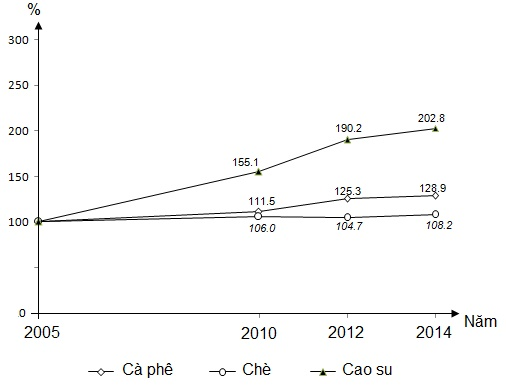
\includegraphics[scale =0.6]{diali01}
\end{center}
Biểu đồ trên thể hiện nội dung nào sau đây?
\datcot[4]
\bonpa
{\sai{Cơ cấu diện tích gieo trồng một số cây công nghiệp lâu năm của nước ta.}}
{\sai{Sự chuyển dịch cơ cấu diện tích gieo trồng một số cây công nghiệp lâu năm của nước ta.}}
{\sai{Quy mô diện tích gieo trồng một số cây công nghiệp lâu năm của nước ta.}}
{\dung{Tốc độ tăng trưởng diện tích gieo trồng một số cây công nghiệp lâu năm của nước ta.}}
\end{question}

\begin{question} %%35
 Cho biểu đồ:
\begin{center}
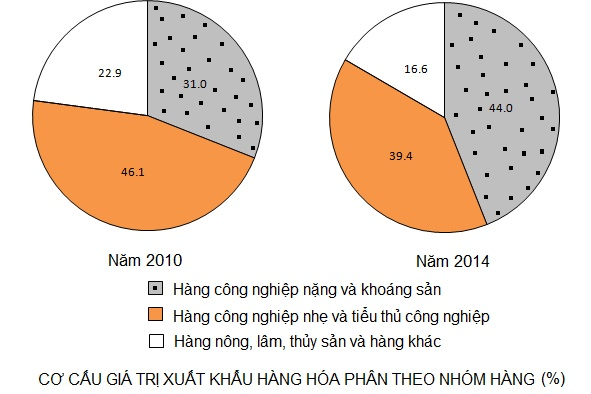
\includegraphics[scale =0.6]{diali02}
\end{center}
Căn cứ vào biểu đồ, hãy cho biết nhận xét nào sau đây đúng về sự thay đổi cơ cấu giá trị xuất khẩu
hàng hóa phân theo nhóm hàng của nước ta năm 2010 và năm 2014?
\datcot[4]
\bonpa
{\sai{Tỉ trọng hàng công nghiệp nặng và khoáng sản giảm.}}
{\sai{Tỉ trọng hàng công nghiệp nhẹ và tiểu thủ công nghiệp tăng.}}
{\sai{Tỉ trọng hàng công nghiệp nặng và khoáng sản luôn lớn nhất.}}
{\dung{Tỉ trọng hàng nông, lâm thuỷ sản và hàng khác luôn nhỏ nhất.}}
\end{question}

\begin{question} %%36
Cho bảng số liệu:\\
\centerline{DIỆN TÍCH GIEO TRỒNG VÀ SẢN LƯỢNG LÚA CẢ NĂM Ở ĐỒNG BẰNG SÔNG HỒNG}
\centerline{VÀ ĐỒNG BẰNG SÔNG CỬU LONG QUA CÁC NĂM}
\begin{center}
\begin{tabular}{| l | l | l | l | l |}\hline
Vùng&Diện tích&(nghìnha)&Sản lượng&lúa (nghìntấn)\\ \cline{2-5}
&2005&2014&2005&2014\\ \hline
Đồng bằng sông Hồng&1186,1&1122,7&6398,4&7175,2\\ \hline
Đồng bằng sông Cửu Long&3826,3&4249,5&19298,5&25475,0\\ \hline
\end{tabular}
\end{center}
\rightline{\textit{(Nguồn: Niên giám thống kê Việt Nam 2015, Nhà xuất bản Thống kê, 2016)}}
Theo bảng trên, hãy cho biết nhận xét nào sau đây \textbf{không đúng} về diện tích và sản lượng lúa cả
năm của Đồng bằng sông Hồng và Đồng bằng sông Cửu Long năm 2005 và năm 2014?
\datcot[4]
\bonpa
{\sai{Diện tích giảm, sản lượng tăng ở Đồng bằng sông Hồng.}}
{\sai{Diện tích tăng, sản lượng tăng ở Đồng bằng sông Cửu Long.}}
{\sai{Sản lượng ở Đồng bằng sông Cửu Long luôn lớn hơn Đồng bằng sông Hồng.}}
{\dung{Diện tích ở Đồng bằng sông Cửu Long tăng nhanh hơn sản lượng.}}
\end{question}

\begin{question} %%37
Ngành công nghiệp chế biến lương thực, thực phẩm của nước ta phát triển chủ yếu dựa vào
\datcot[2]
\bonpa
{\sai{vị trí nằm gần các trung tâm công nghiệp.}}
{\sai{mạng lưới giao thông thuận lợi.}}
{\sai{cơ sở vật chất - kĩ thuật được nâng cấp.}}
{\dung{nguồn nguyên liệu tại chỗ phong phú.}}
\end{question}

\begin{question} %%38
Thế mạnh đặc biệt trong việc phát triển cây công nghiệp có nguồn gốc cận nhiệt và ôn đới ở
Trung du và miền núi Bắc Bộ là do
\datcot[4]
\bonpa
{\sai{đất feralit trên đá phiến, đá vôi chiếm diện tích lớn.}}
{\sai{nguồn nước tưới đảm bảo quanh năm.}}
{\sai{có nhiều giống cây trồng cận nhiệt và ôn đới.}}
{\dung{khí hậu nhiệt đới ẩm gió mùa, có mùa đông lạnh.}}
\end{question}

\begin{question} %%39
Nguyên nhân chủ yếu nào sau đây dẫn đến trình độ thâm canh cao ở Đồng bằng sông Hồng?
\datcot[4]
\bonpa
{\sai{Để giải quyết tình trạng thất nghiệp, thiếu việc làm.}}
{\sai{Do nhu cầu của công nghiệp chế biến lương thực.}}
{\sai{Để có đủ thức ăn cho chăn nuôi lợn và gia cầm.}}
{\dung{Đất chật người đông, nhu cầu lương thực lớn.}}
\end{question}

\begin{question} %%40
 Cho bảng số liệu:\\
\centerline{DIỆN TÍCH CÁC LOẠI CÂY TRỒNG PHÂN THEO NHÓM CÂY}
\rightline{\textit{(Đơn vị: nghìn ha)}}
\begin{center}
\begin{tabular}{| l | l | l |}\hline
\textbf{Năm}&\textbf{2005}&\textbf{2014}\\ \hline
Tổng số&13287,0&14809,4\\ \hline
Cây lương thực&8383,4&8996,2\\ \hline
Cây công nghiệp&2495,1&2843,5\\ \hline
Cây khác&2408,5&2969,7\\ \hline
\end{tabular}
\end{center}
\rightline{\textit{(Nguồn: Niên giám thống kê Việt Nam 2015, Nhà xuất bản Thống kê, 2016)}}
Để thể hiện quy mô diện tích các loại cây trồng và cơ cấu của nó qua hai năm 2005 và 2014, biểu đồ
nào sau đây thích hợp nhất?
\datcot
\bonpa
{\sai{Biểu đồ miền.}}
{\sai{Biểu đồ cột.}}
{\sai{Biểu đồ đường.}}
{\dung{Biểu đồ tròn.}}
\end{question}

\begin{examclosing}
\centerline{-- HẾT --}
\textit{Thí sinh được sử dụng Atlat Địa lí Việt Nam do Nhà xuất bản Giáo dục Việt Nam phát hành từ năm
2009 đến năm 2016.}
\end{examclosing}
 \end{vnmultiplechoice}
\end{document}

